
Now, we describe the \Platform platform, which (1) allows prosumers\footnote{An actor or an agent that can both provide and consume resources.} to post offers and (2) can find a solution to the resource allocation problem in an efficient and trustworthy manner. The actor-based architecture, proposed initially in~\cite{agha1985actors}, has been accepted as a standard model for building distributed applications. The key aspect of an actor-based system are interfaces with well defined execution models~\cite{basu2011rigorous}. 


%\Aron{We need to explain why we do this and why this way.}
%We \change{envision the system as an actor-based distributed architecture}{propose an actor based distributed architecture for the system}, where multiple \Aron{What are the actors?}actors exchange information about their resources and offers. We follow the \Aron{Is this relevant to this conference?} component based software-engineering (CBSE) principle, which has been accepted as a standard practice to develop robust, modular, and maintainable software stacks~\cite{heineman2001component}.  The guiding principles of CBSE are interfaces with well defined execution models \cite{basu2011rigorous}, compositional  semantics \cite{schmidt2003trustworthy}, and model driven analysis \cite{kumar2014colored}. We use an architecture called `Resilient Information Architecture Platform for Smart systems' (RIAPS), developed at our institute~\cite{riaps}. \Aron{How is this related to blockchains?} Each actor in RIAPS is a composition of several libraries that provide (1) a component model that provides a concurrent model of computation for building distributed real-time applications, (2) a messaging framework for facilitating interactions among actors, (3) a resource-management framework for controlling the use of computational resources, (4) a fault-management framework for detecting and mitigating faults in all layers of the system, (5) a security framework to protect the confidentiality, integrity, and availability of system under cyber-attacks, (6) a fault tolerant time synchronization service,  (7) a discovery framework for establishing the network of interacting actors of an application, and (7) a deployment and management framework for the administration and control of the distributed applications from a control room. In this paper, we do not discuss the RIAPS architecture further. Rather, we focus on the architecture of the transaction management platform, which is a distributed application built on top of RIAPS platform. \Aron{It is not actually built on top of RIAPS.}
%\Aron{Can we just omit this paragraph starting from RIAPS? We did not use it, and it might just confuse the reviewers (e.g., how the RIAPS functionality would be integrated with the Ethereum peer-to-peer network.)}

%\subsection{Transaction Management Platform}


\begin{figure}[t]
    \centering
   
% \end{figure}

% \begin{figure}[t]
% \centering
%\resizebox{\columnwidth}{%
\begin{tikzpicture}[x=1.2cm, y=1.2cm, font=\tiny,
  Component/.style={fill=white, draw, align=center, rounded corners=0.1cm, drop shadow={shadow xshift=0.05cm, shadow yshift=-0.05cm, fill=black}},
  Connection/.style={<->, >=stealth, shorten <=0.05cm, shorten >=0.05cm}]

\foreach \pos/\name in {1.6/pros3, 0.8/pros2} { %, 0.0/pros1} {
  \node [Component] (\name) at (\pos - 4, \pos) {Prosumer\\(\texttt{Python}, \texttt{geth})};
}

\node [Component] (dso) at (-1, 2.6) {Directory\\(\texttt{Python}, \texttt{geth})};

\node [Component] (solver) at (-4, 0) {Solver\\(\texttt{Python}, \texttt{CPLEX}, \texttt{geth})};

\fill [fill=black!15] (90:1.5) -- (200:1.5) -- (340:1.5) -- (90:1.5);

\foreach \pos in {90, 200, 340} {
  \node [Component] at (\pos:1.5) {Blockchain\\ miner (\texttt{geth})};
}

\node [Component, dotted] (contract) at (0, 0) {Smart contract\\(\texttt{Solidity})};

\draw [Connection, bend left=62] (solver) to node [midway, left, shift={(-0.25,0)}] {} (dso);

%\draw [Connection, bend left=65] (pros1) to node [midway, left, shift={(-0.25,0)}] {$\emptyset$MQ} (dso);
\draw [Connection, bend left=53] (pros2) to  (dso);
\draw [Connection, bend left=42] (pros3) to (dso);

\draw [Connection, bend right=0] (solver) to node [midway, below left] {Ethereum} (contract);
\draw [Connection, bend right=15] (dso) to (contract);
%\draw [Connection, bend right=0] (pros1) to node [midway, below left] {Ethereum} (contract);
\draw [Connection, bend right=0] (pros2) to (contract);
\draw [Connection, bend right=0] (pros3) to (contract);
\end{tikzpicture}%
%}
\caption{Implementation view of the \Platform. A private Ethereum network (used for testing purposes) is the decentralized computation platform running smart 
\ifExtended
contracts, and the other components interact with the network using the \texttt{geth} Ethereum client. The smart contract is implemented in Solidity, a high-level language for Ethereum.
\else
contracts.
\fi
}
\label{fig:components}
\end{figure}

\begin{figure}[t]
\centering
 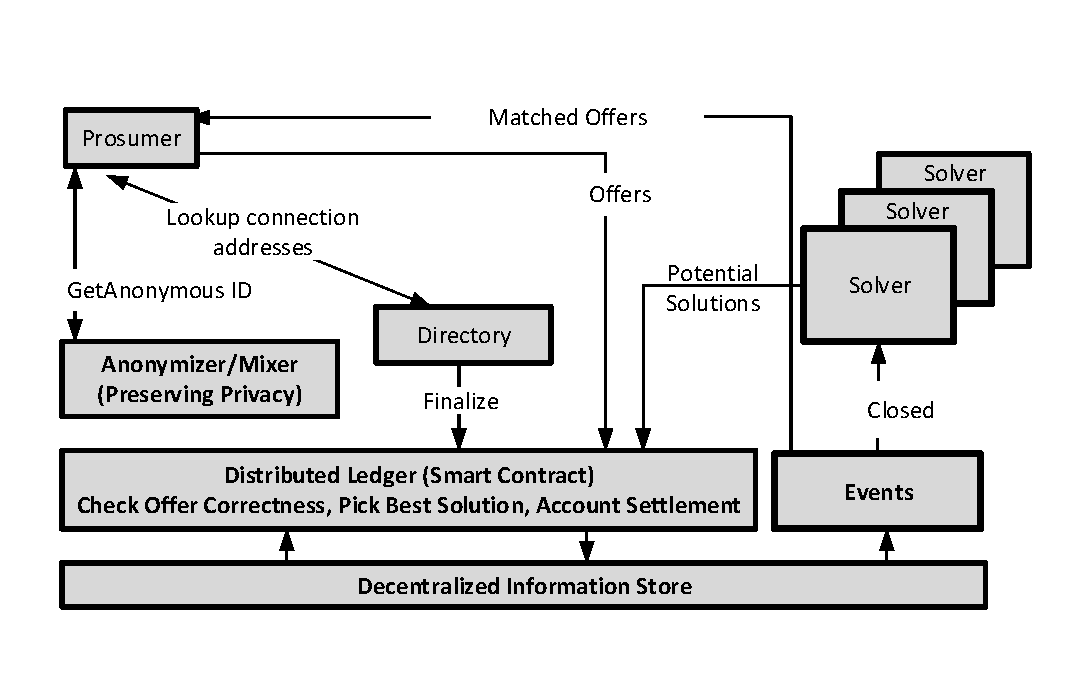
\includegraphics[width=0.9\columnwidth]{BlockchainPaper-update.pdf}
    \caption{Data flow between actors of \Platform. %Information store is part of the blockchain.
        }
    \label{fig:tmp}
\end{figure}


Figure \ref{fig:components} shows the key actors of our transaction management platform,
while
Figure \ref{fig:tmp} describes the data flow between these actors.
A directory actor provides a mechanism to look up connection endpoints, including the address of a deployed smart contract. In our previous work, we  described how to create a decentralized directory service using distributed hash tables~\cite{riaps1}. Therefore, we do not describe the implementation of this service any further in this paper. 
%
Prosumers (i.e., resource providers and consumers) submit offers to the system using functions provided by the smart contract. These functions check the correctness of the offer and then store it in the smart contract. An optional mixer service can be used to obfuscate the identity of the prosumers \cite{serial17}. By generating new anonymous addresses at random periodically, they can prevent other entities from linking the anonymous addresses to their actual identities~\cite{Laszka17,serial17}, thereby keeping their activities private. A set of solvers (pre-configured with constraints and a utility function) can subscribe to smart-contract events, which provide the solvers with information about offers. Solvers run at a pre-configured frequency, compute an optimal resource allocation, and push the assignments into the distributed ledger via the smart contract. An external service director can then choose to frequently operate and finalize the solutions. That is, choose from a number of possible solutions that are available. Once a solution has been finalized, the information is received by the participants via events. 
The following subsections describe the transaction management platform in more detail.
\iffalse
\ad{We need to reinforce the idea that ethereum is just an implementation choice and we believe that in future a proof of stake algorithm should be used for consensus. It does away with wasteful computation and creates a negative incentive for miners to cheat.}
\fi
% Figure \ref{fig:tmp} describes the architecture of our framework. \Aron{Constraints are checked within both the smartcontract and the solver, but not in addition to them.} The orderbook and contracted solutions are stored in a distributed ledger. The automated billing settlement is handled by a smart contract (not described in this paper). \Aron{What is this ``market mechanism''? A collection of services?} The market mechanism is the most important aspect of this platform. It consists of four sub-modules (a) anonymizer/mixer - a cryptographic service that enables the external actors to participate in the market without compromising their privacy, (b) a solver - that is responsible for solving the optimization problem maximizing the configured utility function. Examples of different utility functions were described in the previous section. \Aron{?}The solver is responsible for storing potential solutions to the resource matching problem in the order book, (c) \Aron{Actually, the smart contract does this.} constraint checkers--they ensure the validity of the offers that are stored in the order book and finally (d) a decentralized smart contract that is responsible for finalizing the potential solutions proposed by the solvers. The smart contract is also responsible for running the constraint checkers and then registering the  offers in the \Aron{What is this order book?} order book. 

%\Aron{This seems redundant since the following subsection describes this in more detail.}
%This architecture by design separates the solvers from the smart contract code. There are three reasons for this design decision. The first is that the computation resources required to solve a complex optimization problem are going to be prohibitive to be run within a smart contract. The second reason is that often the state-of-the-art smart-contract languages do not provide native support floating point computations, which are necessary for many solution approaches. The third reason is that this architecture enables us to support a `solver' market where multiple solvers can run in parallel and compete for identifying the best solution (in case they use heuristics to solve the optimization problem). Additionally, it enables us to tolerate solver failures.

\subsection{Scheduling}
\label{sec:scheduling}

Once the system is deployed,
providers and consumers will need to use it repeatedly for finding optimal resource allocations. 
For example, riders and drivers want to find optimal carpooling assignments every day, while users in an energy futures market want to find optimal energy trades every, e.g., 20 minutes.
Consequently, the platform has to gather offers and solve the resource allocation problem at regular time intervals.
Each one of these cycles is divided into two phases.
First, an \emph{offering phase}, in which providers and consumers can post new offers or cancel their existing offers (e.g., if they wish to change their offer based on changes in the market).
Second, a \emph{solving phase}, in which the resource allocation problem is solved for the posted (but not cancelled) offers.
At the end of the second phase, the assignments between providers and consumers are finalized based on the solution.
Then, a new cycle begins with an offering phase.


\subsection{Hybrid Solver Architecture}
\label{sec:solver}
The Resource Allocation Problem described in Section~\ref{sec:problem} can be solved by formulating it as an (integer) linear program (LP): feasibility constraints (Equations~\eqref{eq:feasable1} to~\eqref{eq:feasable4}) and constraint extensions (Section~\ref{sec:extConstr}) can all be formulated as linear inequalities, while the objective function (Equation~\eqref{eq:objective}) as well as the alternative objectives (Section~\ref{sec:extObj}) can be formulated as linear functions. Arguably, we could set up a solver actor that would receive offers from  prosumers, formulate a linear program, and use a state-of-the-art LP-solver (e.g., CPLEX~\cite{cplex2009v12}) to find an optimal solution. However, a simple N-to-1 architecture with N prosumers and 1 solver would suffer from the following problems: 
\begin{itemize}
    \item {\it Lack of trust in solver nodes:} Prosumers would need to trust that the solver is acting selflessly and is providing correct and optimal solutions. 
  %  \item {\it Lack of synchronization between prosumers and the solver:} Prosumers and the solver would have to coordinate the offering and solving phases over a  network. This could be done synchronously, by letting prosumers assume that messages are never lost and letting them actively wait for all messages to arrive in order. However, in practice, we have to allow the possibility of messages being lost and actors losing synchrony. 
    \item {\it Vulnerability of the transaction management platform:} A single solver would be a single point of failure. If it were faulty or compromised, the entire platform would be faulty or compromised.  %A solution will be to use multiple solvers. However, in that case it is important to achieve consensus between the solvers.
    \item {\it Data storage:} For the sake of auditability, information about past offers and allocations should remain available even in case of node failures. 
\end{itemize}


%(a) {\it lack of trust in solver nodes} - how can the prosumers trust that the solver is acting selflessly and is providing correct and optimal solutions. 


%\Aron{I don't understand this sentence. What do you mean by online solutions?} If repeated over a time horizon, an integer linear program solver, such as CPLEX \cite{ref}, end up providing online solutions to the problem. However, there are primarily three problems that arise when we consider \Aron{What architecture?} this architecture (a) lack of trust in solver nodes, (b) asynchrony of the architecture, and (c) failure of the solver nodes. 

A decentralized ledger with distributed information storage and consensus provided by blockchain solutions, such as Ethereum, is an obvious choice for ensuring the auditability of all events and providing distributed trust. However, computation is relatively expensive on blockchain-based distributed platforms\footnote{Further, Solidity, the preferred high-level language for Ethereum, currently lacks built-in support for certain features that would facilitate the implementation of an LP solver, such as floating-point arithmetics.}, solving the trading problem using a block\-chain-based smart contract would not be scalable in practice.
In light of this, we propose a \emph{hybrid implementation approach}, which combines the trustworthiness of blockchain-based smart contracts with the efficiency of more traditional computational platforms.

Thus, the key idea of our hybrid approach is to (1) use a high-performance computer to solve the computationally expensive linear program \emph{off-blockchain} and then (2) use a smart contract to record the solution \emph{on the blockchain}.
To implement this hybrid approach securely and reliably, we must address the following issues.
\begin{itemize}
\item Computation that is performed off-blockchain does not satisfy the auditability and security requirements that smart contracts do. Thus, the results of any off-blockchain computation must be verified %in some way 
by the smart contract before recording them on the blockchain.
\item Due to network disruptions and other errors (including deliberate denial-of-service attacks), the off-blockchain solver might fail to provide the smart contract with a solution on time (i.e., before assignments are supposed to be finalized). Thus, the smart contract must not be strongly coupled to the solver.
\item For the sake of reliability, the smart contract should accept solutions from multiple off-blockchain sources; however, these sources might provide different solutions.
Thus, the smart contract must be able to choose from multiple solutions (some of which may come from a compromised computer).
\end{itemize}



% Section 4.1
% Hybrid Approach for Matching:
% - N solvers (efficient but non-trustworthy platform) + 1 smart contract (trustworthy but not efficient)
% - protocol: each solver may efficiently find a matching and submit it to the smart contract, which selects the best feasible matching
% - trading problem: easy to verify the feasibility of a matching
%   * exact time complexity?
%   * additional constraints might not be easy to verify, depends on the specific trading problem (constraints mentioned above are all easy to verify)
% - workflow (i.e., sequence diagram)
% - system architecture

% Section 4.2
% Privacy:
% - anonymizing mixers and communication anonymity (e.g., onion routing)
